\chapter{Health Bank System} 
\label{chap:generaldesign}
 

%%% ------------- SECTION -------------
\section{Introduction} 

The Healthbank platform shall be a system where the users can administer their health data. Thereby the focus relies completely on these users. Every user is the owner of its data. 
The user controls which applications are allowed to generate data and add entries to its account. The user determines with which doctors, family members and friends record entries are shared with.
Data is generated from different sources and can be illustrated in many different ways. Applications are data sources who provide key-value data plus a tiny bit of metadata for the record entries.

The goal of Healthbank is to build a large database of information related to any kind of health aspects, e.g. diseases, symptoms, drugs, treatment methods, sports activities etc. Once the system is accepted and trusted in by the users, a search engine shall help the users, medical providers and researchers to ask complex queries.  

In the following we will give the reader an overview of the basic functionalities which we think are essential for the system. Then we go into detail and describe how we imagine the architecture and structure of data for Healthbank. Furthermore we describe the technology which shall be used for both client and server side to implement the platform. Finally we will introduce a selected amount of use cases, which define the minimum requirements for the system. \newline

The following list contains the core functionalities which are essential to the desired health system. All additional functionalities may build upon these core functionalities. The word \emph{institute} is used in the following to refer to a group of health care providers such as doctors, doctor`s offices, hospitals, dentists, physiotherapists, psychologists, special clinics and so on. 

\begin{itemize}
	\item Users can create an account and log in and log out of the system. This feature allows users to quickly find and identify their data in the system and protect it from other eyes. 
	\item Users can store, edit and delete their personal health record entries via their system account. This allows full control of a person`s own copy of their health record anytime and anywhere. 
	\item Institutes can create an account and log in and out of the system. In their account they can provide a detailed description about their area of expertise, business hours and whatever they feel useful for the users to know. This helps institutes to be seen by user and for private advertisement. 
	\item A permission system allows users to make their health record or parts of it visible to other users and/or to institutes. With this feature family, friends and institutes can inspect record entries of the user.
	\item Provided the user granted access, institutes can inspect and create new record entries in the health record of a user. This allows e.g. a doctor to upload all the relevant information about the latest visit to the user`s account or gives a hospital insight into important information after an accident happened. 
	\item An entry in the user health record shall be able to contain files (or pointers to) such as x-rays, MRI etc. next to all kind of attributes and text.
	\item A search engine allows to search for users, institutes, record entries, applications and other data stored in the system. This functionality helps to navigate in the system and e.g. to find the right institute in case of specific health problems.
	\item An API provides access to all the core functionalities as well as to possible extensions to the core. This functionality allows the system to grow and external partners to integrate and be part of the system. 
\end{itemize}  

Obviously there are many more featured a system like this could and should provide. As they all build to a certain extent on top of these core functionalities, they are not part of this list. Some of them will be discussed in the remainder of this document.
 

%%% ------------- SECTION -------------
\section{Architecture} 

In this section we describe different constructs in the overall architecture, which we think are essential for a system like Healthbank. Then we will give an overview of how we imagine the general architecture of the system and its components. At the end we will briefly talk about what kind of technologies we expect to be best suited for the architecture.

\subsection{Record Entry}

A record entry is any single piece of data entered into Healthbank. Each entry shall be assigned to and owned by a single user. Examples for entries include results of blood tests, intake of medication, running statistics, what the user ate for lunch, an ECG, a doctor`s visit etc. An entry shall be created via applications in different ways. This includes entering data manually via an application on the Healthbank web site, sending data in through email, creating data by an app on a mobile device or a gadget (e.g. smart running watch) or by bulk loading from an existing database. Entries shall have very few required metadata and otherwise contain all kind of different key-value pairs. Applications shall provide metadata to improve the search experience and to provide information on how to interpret the entry. Entries shall be displayed in many different ways by visualizations.

\subsection{Access Categories} 

The Healthbank access categories shall be very similar to the circles scheme used by Google+ (see chapter \ref{chap:relatedwork}). They shall be the main tool for the management of relations among users and sharing of record entries with others. 
Access categories shall belong to and be maintained by a single user. The user will be able to add other users, patients and/or health care providers to them. Furthermore users shall assign record entries to these categories. All entries which a user assigned to an access category are then visible by all the users in this category. In contrast to social platforms such as Facebook, our access categories are not bidirectional. User $A$ can share data with user $B$ but $B$ does not have to share
anything with $A$. This makes particularly sense if we think about a patient to doctor relation. A patient most certainly wants to share its health record data with its doctor, but a doctor has probably no data entry to share with the patient.

Our system shall be very fine-grained. The user shall be able to decide for every record entry individually, what access categories it is assigned to. The more it shall be possible to share entire folders as well as all data coming from a certain application with an access category. Initially there shall be four predefined, basic categories for family, friends as well as medical and wellness professionals. Since we are dealing with very sensitive data, there is no such thing as a public access category. But there will be a special category called \emph{science}. If a user specifies that an entry is shared with the \emph{science} category, then the user agrees that the entry may be used by scientists (without actually defining who a scientist is) for research purposes.

The system shall allow to create, rename and delete categories. Adding new users to and removing them again from categories as well as assigning categories to entries shall be straight forward. To guarantee this, the developers shall pay special attention to usability aspects for dealing with access categories during the implementation of the system.

\subsection{Folders} 

Some record entries are highly related to each other, e.g. jogging entries or different entries that result from a surgery. Therefore the Healthbank system shall provide folders to help users organize their entries. Similar to a folder in the file system of an operating system, a folder shall contain a set of entries. Folders shall belong to one user and are not visible by others. Similar to access categories it is the user`s responsibility to assign record entries to folders. The assignment to a folder shall either be done fine-grained and individually for every single entry or automatically by assigning folders to applications. In the latter case every new entry by this application will be assigned to the selected folder. \newline
Folders shall not be limited to record entries of one user only. The system will rather allow the users to add data of other users, who shared data with them, as well.

Furthermore, folders shall not only be a set of consolidated record entries but serve as the main way to visualize the information stored in the entries. Therefore folders shall contain visualizations. These will get the entries in the folder as input and are able to illustrate the information in a creative way. 

There shall be three predefined spaces. The \emph{all} space contains the most basic visualization, a simple list, and serves as a feed, much like Twitter or similar networks. This feed lists all the health record entries, events, etc. associated to the user. The other two predefined folders shall be \emph{medical} (contains all the health related information) and \emph{wellness} (contains all the fitness and wellness information). 


\subsection{Market Place} 

One important aspect of the Healthbank system will be to make it extensible and open for third-party providers. These providers shall be able to write applications which allow our users to import data to their record, either manually or from their accounts on the provider`s servers. The more these third-party providers shall be allowed to create applications that visualize the data in the user`s record. Visualizations or illustrations include graphics, statistics and side by side comparisons between users (e.g. jogging data). In order for the users to get to know such applications Healthbank shall provide a market place similar to the application centre on Facebook or the Android Play Store. 

In the following, we define the two types of applications we shall provide with Healthbank. Applications for data generation and import as well as visualizations for data illustration. 

\subsubsection{Applications}

Applications are the main data source for record entries. They shall be small pieces of code that integrate into the GUI and allow the users to add data entries to their health record. The GUI part of an application shall thereby be one of two things. The application can provide a sophisticated GUI or a form where the user can enter data manually. On the other hand, if external providers prefer business to business connections, they can provide a login form or similar. This way we allow the application to identify the user and get the required information.  \newline
Applications shall be listed in the market place where the user will browse through them and click on the desired one. In a detail view the system shall then present the user a description of the application as well as other useful information about it. A review and rating system shall help the users to identify very good applications and give the application providers valuable feedback. This review feature is not essential for a prototype but should be present in an online version of the system. 
From the detail view the user shall be able to install the applications to its account. This will automatically allow the application to get certain user data such as the name, icon and the user identification. This data is needed to make business to business communication possible. 

To illustrate the application concept we present two examples. In a medication application the user can manually add new drugs he or she bought together with time and date, prescription, the drugstore, price etc. To use this 
application the user has to be logged into the system and needs to open the application via the navigation on the page. In the GUI of the application the user can enter the data into a form and save the new entry to its health record. \newline
In a second example a company like Runtastic~\cite{runtastic} (Jogging data) cooperates with Healthbank and provides a simple application. When the user installs this application he or she has to provide the user name and password for their Runtastic account. This data is then transmitted via the application to the Runtastic servers. Now each time the user records a jogging session via Runtastic, their servers will be able to automatically call our API and add a new entry to the user`s health record. This is possible without the need of the user to be logged in. For this business to business communication the security standards shall be especially high.


\subsubsection{Visualizations}

Visualizations are responsible for illustrating data generated by applications. Similar to applications they consist of small pieces of code provided by third-party providers that integrate seamlessly into the folder structure. In contrast to applications they shall not be allowed to add any data to a user`s health record. When loaded in the folder construct the visualization will get the set of record entries assigned to this folder. Using this data they may draw graphs, create statistics, compare different users or visualize the data in any other creative way. Visualizations shall be accessible via the market place. Users shall be able to read a detailed description, to write reviews and to in- and uninstall visualizations to/from their Healthbank account. Furthermore they shall assign them to one or multiple folders. The folder to visualization relation is $n$ to $n$.

As an example one could imagine that Runtastic, after they have built their application for Healthbank, wants to show the user their effort of the last jogging sessions. Hence, they create a visualization and upload it into the market. The user installs the Runtastic visualization and assign it to its jogging folder. When the user now navigates to this folder, the visualization gets the record entries assigned to this folder. It filters out the entries generated by the Runtastic application and shows e.g. a map of the last route, a graph with speed and altitude values and statistics of the user`s overall performance. The more it allows to compare the results with friends of the current user by providing a side by side view of the statistics or by drawing an additional line in the line chart. Obviously this works only with friends who have actively shared their Runtastic data with the user.


\subsection{Health Information Platform}\label{HIP}

Additionally to the user related data the Healthbank system shall implement an information platform. This platform will assemble knowledge about different kind of health data such as e.g. remarks about diseases, medications, nutrition advices or the latest research findings. The platform can have e.g. the form of a wiki. Content shall be provided and edited by doctors and researchers or managed by the Healthbank organization itself. An essential part of the platform must be a drug register (inclusive generic drugs). It is very important on such a platform that the health facts are correct and written in an emotionless way. People tend to be very scared about diseases, so if they search for diseases using their symptoms, the facts should help to acquire knowledge and not increase the hypochondria. As PatientsLikeMe\ref{patientslikeme} and similar platforms showed, that patients like to communicate with people who suffer from the same diseases. Therefore a forum like system or a clever comment system within the wiki needs to be built to give people a platform to discuss their problems and to help each other. A well maintained knowledge database will help to build a certain trust level between the users and Healthbank and motivate the users to visit the site more frequently.
 
Other ideas we had for this platform include a doctors, hospitals and pharmacies register which helps patient to find the specialist closest to them. In this register users can review and comment on the different medical treatments they received. This way users get supported in finding the best doctor for their upcoming surgery and the health providers get feedback on what they do well and where they can still improve.


\subsection{General Architecture}

The general architecture we recommend for the Healthbank system is illustrated in figure \ref{fig:architecture}. The user communicates with the client provided by Healthbank either on a desktop web client or via a mobile version. This client then talks to the Healthbank server REST API, where the data is gathered from the database and sent back to the GUI. For the prototype we only expect to provide a desktop web version for the GUI. A second way to communicate to our server is via an external provider. This way a business to business transmission from the provider`s server to our server`s REST API will add new record entries to the user`s health record. 

% Figure 3.1
\begin{figure}[ht]
%\centering
%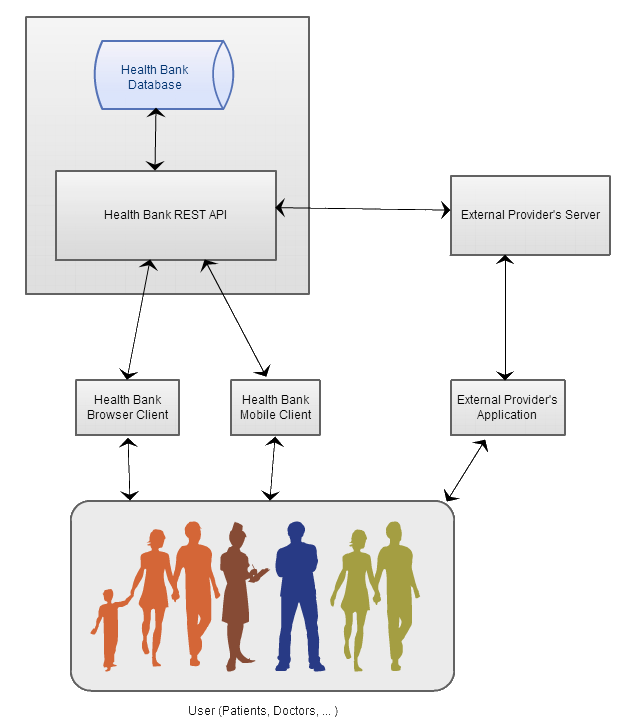
\includegraphics[width=322px,height=363px]{architecture.png}
\makebox[\textwidth][c]{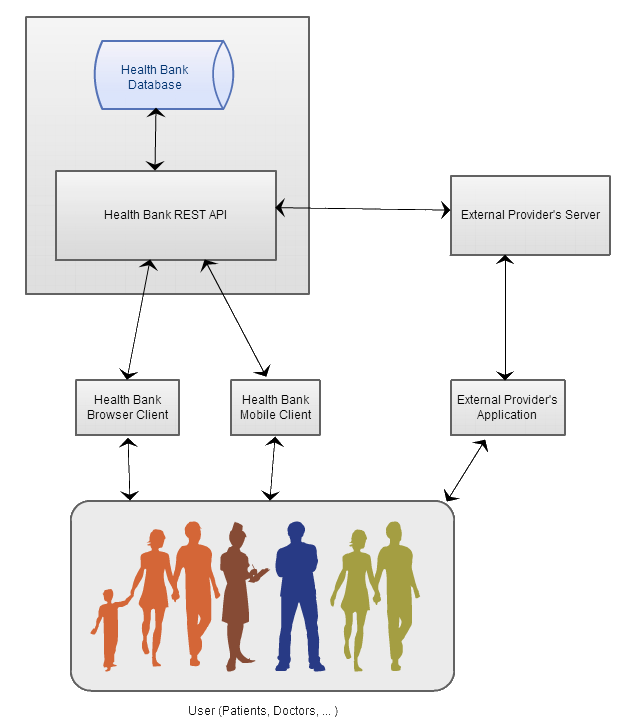
\includegraphics[width=322px,height=363px]{architecture.png}}%
\caption{General architecture of Healthbank system.}
\label{fig:architecture}
\end{figure} 

Figure \ref{fig:ERdiagram} shows an ER diagram of the basic data structure we expect the system to have. This includes the user and institute profiles, record entries and access categories as well as the interaction between them. The diagram shows in particular that it is the user who has control. The user shall create its records and assigns them in a fine-grained way to its access categories. Institutes are very similar to users, they shall create their own records or create record entries for connected users. Institutes shall also create their own access categories for sharing profile information etc. but they will have no way of influencing the user`s access categories. Access categories are always bound to a single user and no one else can view or control them. For the sake of convenience this diagram omits the fact that record entries are effectively generated by applications and inspecting entries is realised via visualizations.
 
% Figure 3.2
\begin{figure}[ht]
%\centering
%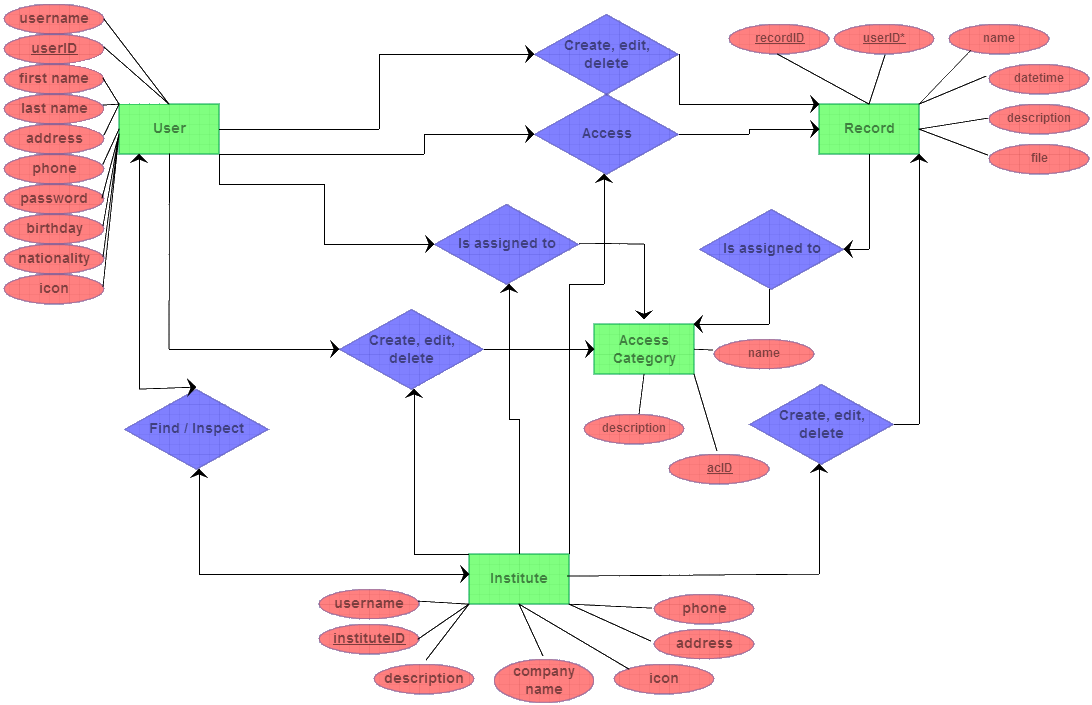
\includegraphics[width=491px,height=317px]{erDiagram.png}
\makebox[\textwidth][c]{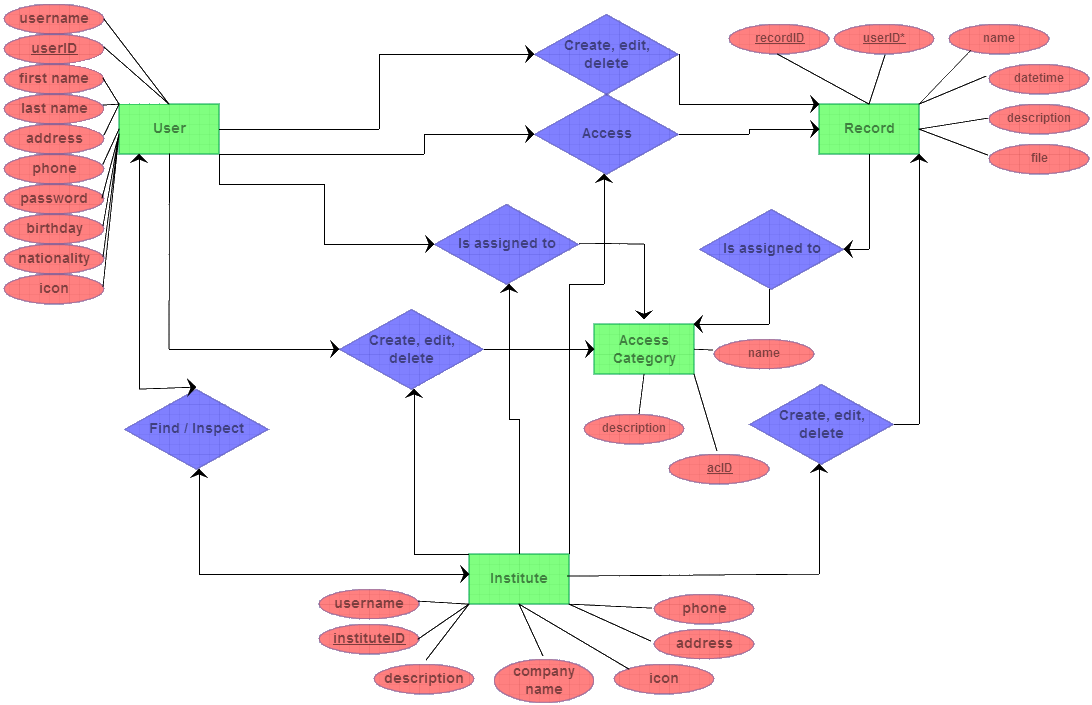
\includegraphics[width=317px,height=317px]{erDiagram.png}}%
\caption{ER diagram of the general setup.}
\label{fig:ERdiagram}
\end{figure} 


\subsection{Technologies} 

The technologies to be used for a system like Healthbank can be very different depending on the knowledge, preferences and expertise of the developers who work on the project. Nevertheless, in the following subsections we shall provide the basic requirements these technologies need to provide to be of use for the Healthbank system. 


\subsubsection{Database} 

The database needs to deal with structured and unstructured data. Apart from the rather structured data of the user accounts, applications, messages etc. the database needs to deal with different kind of record entries. These entries consist of key-value pairs with unpredictable and varying keys. They can be loaded from a SQL database, from a XML or JSON data structure, from an HTML form or even from entire files. To deal with this kind of data we suggest to use a NoSQL database which does not need detailed schema and fixed tables. Because of the JSON data structure, which should work well with a REST API and a JavaScript client, MongoDB would be a reasonable solution. Other possibilities include CouchDB from Apache, eXist, Berkeley DB, or similar databases. 
 
\subsubsection{Server}

The server shall implement a REST API which provides at least functionalities for the user to get access to its data, to store new data and to get into contact with other users. The server needs to connect seamlessly to the database and query it. There are many different approaches which would work perfectly well such as e.g. Java Servlets, PHP, Ruby, ASP.NET or anything alike. 


\subsubsection{Client}

The client is the gate to the user. It shall be user friendly and self-explanatory. If a new user creates an account it shall be very easy and straight forward to get to know the system, install new applications, find friends and upload data. Therefore the client shall be either a website with well-known patterns or a native application for a smartphone or tablet. Also a rich desktop application is conceivable. Regarding technologies the engineers implementing a client shall focus on user friendliness and a modern UI which supports animations, drag-and-drop interaction as well as touch input. For the prototype we expect it to have a desktop web application preferably built in HTML 5 and any kind of JavaScript framework.

 

%%% ------------- SECTION -------------
\section{Use Cases} 
\label{usecase}

The following table \ref{tab:usecaseTable} shows a subset of the use cases we derived for the Healthbank system. The document which contains all of the about fifty use cases is provided with the source code of the prototype. All the use cases with an id of $1.x$ in this document are applicable for both normal users and institute users. Whereas the use cases with an id of $2.x$ are only applicable for institute
users. In the table the shortcut \emph{app} stands for applications, \emph{HR} for health record and \emph{AC} for access category.
\newpage

\begin{table}[ht]
  \centering
	\begin{tabular}{c l l}
	Id & Use Case & Description \\
	\hline
	\\
	1.1 & Register user & Create and register a new user to the system. \\ 
	1.2 & Login user &  A registered user can log into the system.\\
	1.3 & Logout user &  A logged in user can log out of the system.\\
	1.4 & Add entry to HR & A user can manually add entries to its HR. \\
	1.5 & View HR & A user can view all the entries in its HR. \\
	1.6 & Edit entry in HR & A user can change the data in an entry of its HR. \\
	1.7 & Delete entry in HR & A user can delete an entry in its HR. \\
	1.8 & Change personal settings & A user can change its profile settings. \\
	1.9 & Search & A user can search entries, other users and apps. \\
	1.10 & View record of other user & A user can view shared entries of another user.  \\
	1.11 & Create AC & A user can create AC to control data sharing. \\
	1.12 & Add person to AC & Users can add other users to its ACs to share  \\
	 & & data with them. \\
	1.13 & Remove person from AC & Users can remove other users from ACs. \\
	1.14 & Change entries AC assignment & Users can for each entry change its assignment  \\
	 & & to ACs. \\
	1.15 & Edit AC & The metadata of an AC can be changed. \\
	1.16 & Delete AC & An AC can be deleted. \\
	1.17 & Group entries into folders & Multiple entries can be assigned to folders for  \\
	 & & a better overview. \\
	1.18 & Install app to profile & Users shall be able to install external apps  \\
	 & & from a market. \\
	1.19 & Remove app from profile & Users shall be able to uninstall installed apps. \\
	1.20 & Send message to other user & Users can send messages to other users. \\
	1.21 & Delete profile & Users shall be able to remove their profile from  \\
	 & & the system \\
	\hline
	\\
	2.1 & Institute adds entry to user & An institute shall be able to add entries to users,  \\
	 & & if they allow. \\
	2.2 & Institute profile different & The profile of an institute user shall be different  \\
	 & & then of a normal user. \\
	2.3 & Query engine & Selected research institutes shall be able to use  \\
	 & & a sophisticated search engine for the big data. \\
	2.4 & Add app to system & Institute users shall be able to add new apps  \\
	 & & to the system. \\
	2.5 & Edit app data & The app author shall be able to update and change  \\
	 & & app information. \\
	2.6 & Remove application & The app author shall be able to remove an app  \\
	 & & from the system. \\
	2.7 & App adds entry to user & Apps shall be able to add new entries to user`s  \\
	 & & record, if they allow. \\
	2.8 & App illustrates record & Apps shall be able to visualize a set of entries in the  \\
	 & & user record, if they allow. \\
	\end{tabular}
	\caption{A subset of the use cases for Healthbank}
  \label{tab:usecaseTable}
\end{table}
 
%%% Local Variables: 
%%% mode: latex 
%%% TeX-master: "thesis" 
%%% End:
 
